\documentclass[onecolumn, 12 pt, doublespacing, fullpage, a4paper]{report}

\usepackage[utf8]{inputenc}
\usepackage[vietnamese]{babel}
\usepackage{amsmath}

\usepackage[hyphens]{url}
\usepackage{hyperref}

\usepackage{amssymb}
\usepackage{amsthm}
\usepackage{verbatim}
\usepackage{sectsty}
\usepackage{xhfill}
\usepackage{wrapfig}
\usepackage{scrextend}
\usepackage{fancyhdr}
\usepackage{array}
\usepackage{cases}
\usepackage{parallel}
\usepackage{pgf-pie} %vẽ biểu đồ hình tròn
\usepackage{graphicx} %chen hình ảnh
\usepackage{float} %đặt hình ảnh ở vị trí mong muốn
%vẽ hộp
\usepackage{tcolorbox} 
%vẽ sơ đồ
\usepackage{tikz}
\changefontsizes{13pt}
\usepackage[lmargin=35mm, rmargin=25mm, vmargin=25mm, headsep=2.5mm]{geometry}

\usepackage{tabularx} %bảng
\usepackage{xltabular} % Hỗ trợ bảng dài tự động ngắt trang
\usepackage{multirow}
\usepackage{diagbox}
\usepackage{makecell}

\usepackage{enumitem}

\usepackage{setspace} %chỉnh giãn dòng riêng đoạn văn \begin{spacing}{1.2} \end{spacing}

\renewcommand{\baselinestretch}{1.3} % baseline stretch giãn dòng
\setlength{\parskip}{0.8em}
\setlength{\parindent}{0.07pt}

\begin{document}
%----------BÌA-----------%
\begin{titlepage}

    \centering
    
    \textbf{\large ĐẠI HỌC HUẾ}\\
    \textbf{\large TRƯỜNG ĐẠI HỌC SƯ PHẠM}\\[-0.5cm] %hoặc \vspace{-0.5cm} %chỉnh dòng dưới sát dòng trên
    \rule{5cm}{0.5pt} % Đường gạch ngang nhỏ dưới tên trường

    
    \vspace{2cm}
    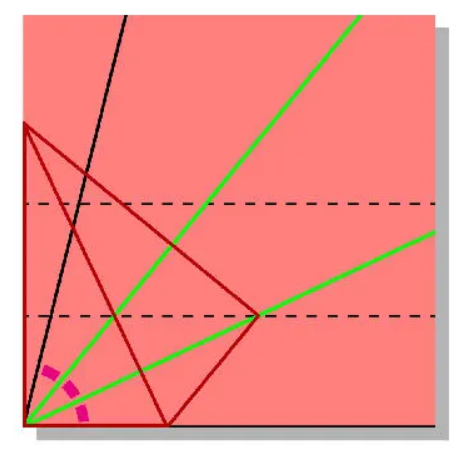
\includegraphics[scale=0.8]{photos/origami.PNG}
    
    \vspace{2cm}
    \textbf{\LARGE ORIGAMI \\ VÀ SỨC MẠNH GIẢI QUYẾT\\BÀI TOÁN CỔ ĐIỂN}
    
    
    
    \vspace{2cm}
    {\large Giáo viên hướng dẫn: } Nguyễn Đăng Minh Phúc\\
    {\large Sinh viên thực hiện: } Trần Thị Thanh Thảo\\
    {\large MSV: }23S7010008
    
    \vfill
    \textbf{\large Thành phố Huế, 09/2026}
\end{titlepage}
%------------BÌA----------%


\tableofcontents
\chapterfont{\fontsize{14}{20}\selectfont}   % font size and baseline stretch
\sectionfont{\fontsize{14}{15}\selectfont}
\subsectionfont{\fontsize{14}{15}\selectfont}
\subsubsectionfont{\fontsize{14}{15}\selectfont}

    
\pagestyle{fancy} % adds a line at the top of every page, except title-page
\fancyhead{} \fancyfoot{} % for header and footer
\fancyhead[CO,CE]{\thepage}    % center odd and even page number

%centering the page numbers with text body
\fancyheadoffset[L]{0.01mm}
\renewcommand{\headrulewidth}{0pt}


%The following code changes the empty vertical space above a new chapter title. It sets it from 50pt to 20pt
\makeatletter
\patchcmd{\@makechapterhead}{50\p@}{20pt}{}{}
\patchcmd{\@makeschapterhead}{50\p@}{20pt}{}{}
\makeatother
%end of modification


%đánh số trang ở trên giữa trang
\fancypagestyle{plain}{
\fancyhf{} %clear all header and footer fields
\fancyhead[C]{\thepage} %puts number on top center of the page
\renewcommand{\headrulewidth}{0pt}
\renewcommand{\footrulewidth}{0pt}}





\include{01-Mở đầu}

%để trống 1 trang (k có số trang)
\newpage
\null
\thispagestyle{empty}
\newpage

\begin{center}
{{\bf\fontsize{14pt}{14.5pt}\selectfont 
MỞ ĐẦU}}
\end{center}
\addcontentsline{toc}{chapter}{MỞ ĐẦU}



Origami truyền thống trong văn hóa dân gian Nhật Bản vốn được biết đến như nghệ thuật tạo hình từ một tờ giấy vuông phẳng, không dùng kéo hay hồ dán. Tuy nhiên, dưới lăng kính toán học hiện đại nửa cuối thế kỷ 20, mỗi nếp gấp thẳng thực chất là sự hiện thực hóa của một thao tác hình học xác định. Khi gấp một tờ giấy, ta đang thực hiện các phép biến hình đối xứng trục, tìm giao điểm và dựng đường bao.

Trong hơn 2.000 năm, hình học cổ điển bị chi phối bởi các tiên đề Euclid cùng hai công cụ chuẩn tắc: thước kẻ không chia vạch và compa. Hệ công cụ này đã đặt ra hai bài toán dựng hình kinh điển thời Hy Lạp cổ đại:
\begin{enumerate}
    \item \textbf{Chia ba một góc:} Chia một góc phẳng bất kỳ thành ba phần bằng nhau.
    \item \textbf{Nhân đôi khối lập phương (Bài toán Delian):} Dựng cạnh của khối lập phương có thể tích gấp đôi thể tích khối lập phương ban đầu (tương đương dựng đoạn thẳng có độ dài $\sqrt[3]{2}$).
\end{enumerate}

Vào thế kỷ 19, lý thuyết Galois và đại số trừu tượng của Pierre Wantzel (1837) cùng Ferdinand von Lindemann (1882) đã chứng minh dứt khoát rằng cả ba bài toán trên đều bất khả thi nếu chỉ dùng thước kẻ và compa. 

Tuy nhiên, giới hạn đó không thuộc về bản chất của hình học, mà thuộc về sự giới hạn của chính hai công cụ cổ điển. Bằng việc hệ thống hóa các thao tác gấp qua hệ 7 tiên đề Huzita--Hatori, Origami đã chứng minh năng lực vượt trội: giải quyết trọn vẹn bài toán chia ba góc và nhân đôi khối lập phương. 

Tiểu luận này tập trung làm rõ:
\begin{itemize}
    \item Giới hạn đại số của thước kẻ -- compa so với năng lực giải phương trình bậc ba của Origami thông qua Tiên đề 6.
    \item Trực quan hóa hình học bản chất của Tiên đề 6: bài toán dựng tiếp tuyến chung của hai đường parabol.
    \item Hướng dẫn thực nghiệm, đo đạc sai số và phân tích hình học cho hai quy trình gập kinh điển của Abe Hisashi và Peter Messer.
\end{itemize}
\chapter{Giới hạn của Thước kẻ -- Compa và Tiên đề 6}

\section{Giới hạn đại số của hệ dựng hình Euclid}

Trong hình học Euclid phẳng, mọi phép dựng hình bằng thước kẻ không chia độ và compa đều quy về việc thực hiện hữu hạn các thao tác cơ bản sau:
\begin{enumerate}
    \item Tìm giao điểm của hai đường thẳng (tương đương giải hệ hai phương trình bậc nhất).
    \item Tìm giao điểm của một đường thẳng và một đường tròn (tương đương giải hệ gồm một phương trình bậc nhất và một phương trình bậc hai).
    \item Tìm giao điểm của hai đường tròn (tương đương giải hệ hai phương trình bậc hai).
\end{enumerate}

Về mặt đại số, nếu xuất phát từ một trường số cơ sở $\mathbb{Q}$, mỗi phép dựng bằng thước kẻ và compa chỉ cho phép ta mở rộng trường số bằng cách khai căn bậc hai. Nghĩa là, nếu một số $\alpha$ dựng được bằng thước kẻ và compa, thì bậc của trường mở rộng $[\mathbb{Q}(\alpha) : \mathbb{Q}]$ phải có dạng:
\begin{equation}
    [\mathbb{Q}(\alpha) : \mathbb{Q}] = 2^k \quad (k \in \mathbb{N}).
\end{equation}

Đối với bài toán nhân đôi khối lập phương, ta cần dựng đại lượng $x = \sqrt[3]{2}$, là nghiệm của đa thức bất khả quy $x^3 - 2 = 0$ trên $\mathbb{Q}$. Bậc mở rộng tương ứng là:
\begin{equation}
    [\mathbb{Q}(\sqrt[3]{2}) : \mathbb{Q}] = 3 \neq 2^k.
\end{equation}

Đối với bài toán chia ba góc, xét góc $\theta = 60^\circ$, việc chia ba góc này quy về việc tính $x = \cos(20^\circ)$. Dùng công thức nhân ba $\cos(3\theta) = 4\cos^3\theta - 3\cos\theta$, ta có phương trình:
\begin{equation}
    8x^3 - 6x - 1 = 0.
\end{equation}
Đa thức này bất khả quy trên $\mathbb{Q}$, do đó $[\mathbb{Q}(\cos 20^\circ) : \mathbb{Q}] = 3 \neq 2^k$.

Vì $3$ không phải là lũy thừa của $2$, cả hai bài toán đều hoàn toàn bất khả thi trong hệ dựng hình Euclid.

\section{Hệ 7 tiên đề Huzita--Hatori trong Origami}

Hệ thống toán học của Origami được hoàn thiện nhờ Humiaki Huzita (1989) và Koshiro Hatori (2001), bao gồm 7 tiên đề xác định cách tạo ra một nếp gấp thẳng duy nhất từ các điểm và đường thẳng cho trước:

\begin{enumerate}
    \item \textbf{Tiên đề 1:} Cho hai điểm $P_1, P_2$, có duy nhất một nếp gấp đi qua cả hai điểm (tương đương kẻ đường thẳng qua 2 điểm).
    \item \textbf{Tiên đề 2:} Cho hai điểm $P_1, P_2$, có duy nhất một nếp gấp đưa $P_1$ trùng vào $P_2$ (dựng đường trung trực).
    \item \textbf{Tiên đề 3:} Cho hai đường thẳng $L_1, L_2$, có thể gấp đưa $L_1$ trùng vào $L_2$ (dựng đường phân giác).
    \item \textbf{Tiên đề 4:} Cho điểm $P_1$ và đường thẳng $L_1$, có duy nhất một nếp gấp đi qua $P_1$ và vuông góc với $L_1$ (dựng đường vuông góc).
    \item \textbf{Tiên đề 5:} Cho hai điểm $P_1, P_2$ và đường thẳng $L_1$, có thể gấp đưa $P_1$ nằm trên $L_1$ sao cho nếp gấp đi qua $P_2$ (tương đương dựng giao điểm của đường tròn và đường thẳng).
    \item \textbf{Tiên đề 6:} Cho hai điểm $P_1, P_2$ và hai đường thẳng $L_1, L_2$, có thể tạo một nếp gấp đưa đồng thời $P_1$ lên $L_1$ và $P_2$ lên $L_2$.
    \item \textbf{Tiên đề 7:} Cho điểm $P_1$ và hai đường thẳng $L_1, L_2$, có thể tạo một nếp gấp đưa $P_1$ lên $L_1$ sao cho nếp gấp vuông góc với $L_2$.
\end{enumerate}

Các Tiên đề từ 1 đến 5 và Tiên đề 7 chỉ tương đương với các phép toán giải phương trình bậc nhất và bậc hai. Riêng \textbf{Tiên đề 6} mang lại bước nhảy vọt về năng lực dựng hình.

\section{Bản chất hình học của Tiên đề 6: Tiếp tuyến chung của hai Parabol}

Xét thao tác gấp một điểm $P$ lên một đường thẳng $L$ bởi nếp gấp $T$:
\begin{itemize}
    \item Nếp gấp $T$ chính là đường trung trực của đoạn nối điểm $P$ với ảnh $P'$ của nó trên $L$.
    \item Theo định nghĩa quỹ tích hình học, đường thẳng $T$ luôn tiếp xúc với một parabol có tiêu điểm (focus) là $P$ và đường chuẩn (directrix) là $L$.
\end{itemize}

Khi thực hiện Tiên đề 6:
\begin{itemize}
    \item Thao tác đưa $P_1$ lên $L_1$ đòi hỏi nếp gấp $T$ phải tiếp xúc với Parabol $\mathcal{P}_1$ (tiêu điểm $P_1$, đường chuẩn $L_1$).
    \item Thao tác đồng thời đưa $P_2$ lên $L_2$ đòi hỏi $T$ tiếp xúc với Parabol $\mathcal{P}_2$ (tiêu điểm $P_2$, đường chuẩn $L_2$).
\end{itemize}

Do đó, nếp gấp $T$ chính là \textbf{tiếp tuyến chung} của hai đường parabol $\mathcal{P}_1$ và $\mathcal{P}_2$.

\begin{figure}[H]
    \centering
    \begin{tikzpicture}[scale=1.1, >=stealth]
        % --- Khung nền tờ giấy Origami ---
        \fill[gray!5] (-2,-2) rectangle (5,5);
        \draw[thick, gray!60] (-2,-2) rectangle (5,5);

        % --- Đường chuẩn L1 và L2 ---
        \draw[very thick, blue!80!black] (-1, -1.8) -- (-1, 4.8) node[above] {\small $L_1$ (chuẩn của $\mathcal{P}_1$)};
        \draw[very thick, red!80!black] (-1.8, -1) -- (4.8, -1) node[right] {\small $L_2$ (chuẩn của $\mathcal{P}_2$)};

        % --- Tiêu điểm P1 và P2 ---
        \coordinate (P1) at (1, 2);
        \coordinate (P2) at (2, 1);
        \fill[blue!90!black] (P1) circle (2.2pt) node[above left] {$P_1$};
        \fill[red!90!black] (P2) circle (2.2pt) node[below right] {$P_2$};

        % --- Hai đường Parabol P1 và P2 ---
        % Parabol P1: Tiêu điểm (1,2), đường chuẩn x = -1 -> Đỉnh (0,2), pt: x = (y-2)^2 / 4
        \draw[thick, blue!65, domain=-0.8:4.8, smooth, variable=\y] 
            plot ({((\y-2)^2)/4}, \y);
        \node[blue!80!black, font=\footnotesize] at (3.5, 4.4) {$\mathcal{P}_1$ (tiêu điểm $P_1$, chuẩn $L_1$)};

        % Parabol P2: Tiêu điểm (2,1), đường chuẩn y = -1 -> Đỉnh (2,0), pt: y = (x-2)^2 / 4
        \draw[thick, red!65, domain=-0.8:4.8, smooth, variable=\x] 
            plot (\x, {((\x-2)^2)/4});
        \node[red!80!black, font=\footnotesize] at (4.4, 2.0) {$\mathcal{P}_2$ (tiêu điểm $P_2$, chuẩn $L_2$)};

        % --- Nếp gấp T: Tiếp tuyến chung đối xứng x + y = 1 (y = -x + 1) ---
        % Tiếp xúc P1 tại (1, 0) và P2 tại (0, 1)
        \draw[very thick, teal, dashed, domain=-1.6:2.6] 
            plot (\x, {-\x + 1});
        \node[teal!90!black, font=\bfseries, rotate=-45] at (2.2, -0.8) {Nếp gấp $T$ (tiếp tuyến chung)};

        % --- Các điểm tiếp xúc của T với 2 Parabol ---
        \coordinate (Touch1) at (1, 0);
        \coordinate (Touch2) at (0, 1);
        \fill[teal] (Touch1) circle (2pt) node[below left, font=\scriptsize] {Tiếp xúc $\mathcal{P}_1$};
        \fill[teal] (Touch2) circle (2pt) node[above right, font=\scriptsize] {Tiếp xúc $\mathcal{P}_2$};

        % --- Minh họa điểm ảnh P1' in L1 và P2' in L2 qua nếp gấp ---
        \coordinate (P1_prime) at (-1, 0);
        \coordinate (P2_prime) at (0, -1);
        \fill[blue!50!black] (P1_prime) circle (1.8pt) node[left] {$P'_1 \in L_1$};
        \fill[red!50!black] (P2_prime) circle (1.8pt) node[below] {$P'_2 \in L_2$};

        % Đường gióng phản xạ vuông góc với nếp gấp T
        \draw[densely dotted, blue!70] (P1) -- (P1_prime);
        \draw[densely dotted, red!70] (P2) -- (P2_prime);
    \end{tikzpicture}
    \caption{Cơ sở hình học của Tiên đề 6: Nếp gấp $T$ đưa đồng thời $P_1 \to L_1$ và $P_2 \to L_2$ tiếp xúc với $\mathcal{P}_1$ tại $(1,0)$ và $\mathcal{P}_2$ tại $(0,1)$, trở thành tiếp tuyến chung của hai parabol.}
    \label{fig:axiom6_tangent_steps}
\end{figure}

\section{Ý nghĩa đại số: Giải phương trình bậc ba}

Giả sử nếp gấp $T$ có hệ số góc là $m$. Điều kiện để một đường thẳng tiếp xúc với một parabol bậc hai dẫn đến một phương trình liên hệ giữa $m$ và các tham số của parabol.

Khi xét đồng thời hai parabol có trục không song song, việc tìm tiếp tuyến chung dẫn đến việc giải một hệ phương trình mà sau khi khử tham số sẽ thu được một \textbf{phương trình bậc ba} đối với hệ số góc $m$:
\begin{equation}
    a_3 m^3 + a_2 m^2 + a_1 m + a_0 = 0 \quad (a_3 \neq 0).
\end{equation}

Hai parabol có thể có tối đa 3 tiếp tuyến chung thực, tương ứng với tối đa 3 nghiệm thực của phương trình bậc ba. Thao tác gập giấy vật lý trong Tiên đề 6 cho phép ta trượt và xoay tờ giấy liên tục cho đến khi hai điểm chạm đồng thời vào hai đường thẳng, tức là trực tiếp tìm ra nghiệm thực của phương trình bậc ba mà không cần công thức Cardano phức tạp.


Vì trường số dựng được bởi Origami có thể mở rộng bậc 3, ta hoàn toàn có thể xây dựng các trường mở rộng có dạng:
\begin{equation}
    [\mathbb{K} : \mathbb{Q}] = 2^a \cdot 3^b \quad (a, b \in \mathbb{N}).
\end{equation}
Đây chính là lý do toán học giải thích vì sao Origami giải quyết được triệt để cả bài toán chia ba góc và nhân đôi khối lập phương.
\chapter{Thực nghiệm giải quyết 2 bài toán kinh điển}
\section{Thực nghiệm 1: Chia ba một góc bất kỳ}
\subsection{Quy trình}
Phương pháp do Abe Hisashi công bố năm 1980 cho phép chia đều một góc nhọn bất kỳ thành ba phần bằng nhau bằng việc kết hợp các nếp gấp song song và Tiên đề 6.

\textbf{Bước 1: Chuẩn bị góc và hai nếp gấp song song}

Xét một tờ giấy hình vuông cạnh $a$. Đặt góc nhọn cần chia ba $\angle AOB = \theta$ tại đỉnh dưới cùng bên trái $O(0,0)$, với cạnh $OB$ nằm trùng trên mép đáy của tờ giấy.

\begin{enumerate}
    \item Dựng nếp gấp ngang $L_1$ song song với mép đáy $L_0$, cách mép đáy một khoảng cách $d$ tùy ý.
    \item Gập mép đáy $L_0$ đè lên nếp gấp $L_1$ để tạo tiếp nếp gấp ngang thứ hai $L_2$ song song với $L_1$, sao cho khoảng cách giữa $L_1$ và $L_2$ cũng bằng đúng $d$.
    \item Đánh dấu giao điểm của nếp gấp $L_1$ với mép đứng bên trái là điểm $P$.
\end{enumerate}

\begin{figure}[H]
    \centering
    \begin{tikzpicture}[scale=0.95, >=stealth]
        % Tờ giấy vuông
        \draw[thick, fill=gray!5] (0,0) rectangle (6,6);
        \node[below left] at (0,0) {$O$};
        
        % Cạnh góc và tia OA
        \draw[very thick, black] (0,0) -- (6,0) node[below left] {$B$};
        \draw[very thick, black] (0,0) -- (4.24,5.05) node[above right] {$A$};
        \draw[domain=0:50, ->] (0.9,0) arc (0:50:0.9);
        \node at (1.2,0.45) {$\theta$};

        % Hai đường song song L1 và L2
        \draw[thick, blue!80, dashed] (0,1.2) -- (6,1.2) node[right] {$L_1$};
        \draw[thick, blue!80, dashed] (0,2.4) -- (6,2.4) node[right] {$L_2$};

        % Điểm P và các khoảng cách d
        \coordinate (P) at (0,1.2);
        \fill[blue!90!black] (P) circle (2pt) node[left] {$P$};
        
        \draw[<->, gray!80] (5.2, 0) -- (5.2, 1.2) node[midway, fill=gray!5, inner sep=1pt] {\footnotesize $d$};
        \draw[<->, gray!80] (5.2, 1.2) -- (5.2, 2.4) node[midway, fill=gray!5, inner sep=1pt] {\footnotesize $d$};
    \end{tikzpicture}
    \caption{Bước 1: Thiết lập góc $\theta$ tại đỉnh $O$ và dựng hai dải giấy song song cùng bề rộng $d$.}
    \label{fig:abe_step1}
\end{figure}

\textbf{Bước 2: Thao tác mấu chốt theo Tiên đề 6}

Áp dụng Tiên đề 6 cho hệ gồm hai điểm $\{O, P\}$ và hai đường thẳng $\{OA, L_2\}$:
\begin{itemize}
    \item Uốn cong tờ giấy và điều chỉnh duy nhất một nếp gấp $T$ sao cho:
    \begin{itemize}
        \item Đỉnh $O$ thuộc $L_1$
        \item Điểm mấu chốt $P$ tiếp xúc lên $OA$ tại điểm $P'$.
    \end{itemize}
    \item Miết cố định nếp gấp $T$.
\end{itemize}

\begin{figure}[H]
    \centering
    \begin{tikzpicture}[scale=1.05, >=stealth]
        % --- Khung tờ giấy hình vuông Origami ---
        \draw[thick, fill=gray!4] (0,0) rectangle (6,6);
        \coordinate (O) at (0,0);
        \coordinate (B) at (6,0);
        \node[below left, font=\bfseries] at (O) {$O$};
        \node[below left] at (B) {$B$};
        \draw[thick, black] (O) -- (B);

        % --- Hai đường gióng song song L1 và L2 ---
        % L1 ở cao độ y = 1.4, L2 ở cao độ y = 2.8
        \draw[thick, blue!60!black, dashed] (0, 1.4) -- (6, 1.4)
            node[right, font=\footnotesize\bfseries, blue!80!black] {$L_1$};
        \draw[thick, blue!60!black, dashed] (0, 2.8) -- (6, 2.8)
            node[right, font=\footnotesize\bfseries, blue!80!black] {$L_2$};

        % --- Điểm P nằm ở giao của L2 và lề mép trái: (0, 2.8) ---
        \coordinate (P) at (0, 2.8);
        \fill[blue!90!black] (P) circle (2.2pt);
        \node[left, font=\bfseries, blue!90!black] at (P) {$P$};

        % Đỉnh O ban đầu tại góc trái dưới (0,0)
        \fill[black] (O) circle (2.2pt);

        % --- Tia OA (tạo góc theta ~ 50 độ từ gốc O) ---
        \coordinate (A) at (4.2, 5.0);
        \draw[thick, black] (O) -- (A) node[above right] {$A$};

        % --- Nếp gấp Tiên đề 6: T ---
        \coordinate (Fold1) at (0, 4.4);
        \coordinate (Fold2) at (4.6, 0);
        \draw[very thick, teal, dashdotted] (Fold1) -- (Fold2);
        \node[teal!90!black, font=\footnotesize\bfseries, fill=white, inner sep=2pt, draw=teal!40, rounded corners=2pt, rotate=-44] 
            at (3.4, 1.2) {Nếp gấp $T$};

        % --- Các điểm chạm sau khi gập: O' in L1 và P' in OA ---
        % O' nằm chính xác trên L1 (y = 1.4)
        \coordinate (Oprime) at (2.2, 1.4);
        % P' nằm trên đường chứa tia OA
        \coordinate (Pprime) at (2.6, 3.1);

        \fill[red!80!black] (Oprime) circle (2.2pt);
        \node[red!80!black, font=\footnotesize\bfseries, below right, fill=white, inner sep=1.5pt, rounded corners=1pt] 
            at (2.2, 1.3) {$O' \in L_1$};

        \fill[purple!80!black] (Pprime) circle (2.2pt);
        \node[purple!80!black, font=\footnotesize\bfseries, above left, fill=white, inner sep=1.5pt, rounded corners=1pt] 
            at (2.55, 3.25) {$P' \in OA$};

        % --- Mũi tên mô phỏng chuyển động gập ---
        \draw[->, thick, red!80!black, bend right=20] 
            (0.15, 0.1) to node[midway, below right, font=\footnotesize] {gập $O \to L_1$} (2.05, 1.3);

        \draw[->, thick, blue!80!black, bend left=20] 
            (0.15, 2.9) to node[midway, above left, font=\footnotesize] {gập $P \to OA$} (2.45, 3.2);
    \end{tikzpicture}
    \caption{Bước 2: Áp dụng Tiên đề 6 đưa đồng thời đỉnh $O$ chạm vào đường $L_1$ (tại $O'$) và điểm $P$ trên lề đường $L_2$ chạm vào tia $OA$ (tại $P'$) qua nếp gấp $T$.}
    \label{fig:abe_step2}
\end{figure}

   
\textbf{Bước 3: Mở nếp gập và thu nhận ba góc bằng nhau}

Khi mở tờ giấy ra:
\begin{enumerate}
    \item Nếp gấp T cắt $L_1$ tại $K$.
    \item Gấp theo đường thẳng $OK$.
    \item Gấp mép $OB$ trùng với $OK$
    \item Góc $\angle AOB$ ban đầu bị phân chia chính xác thành ba góc bằng nhau:
    \begin{equation}
        \theta_1 = \theta_2 = \theta_3 = \frac{\theta}{3}.
    \end{equation}
\end{enumerate}

\begin{figure}[H]
    \centering
    \begin{tikzpicture}[scale=1.1, >=stealth]
        % --- Khung tờ giấy hình vuông Origami ---
        \draw[thick, fill=gray!4] (0,0) rectangle (6,6);
        \coordinate (O) at (0,0);
        \coordinate (B) at (6,0);
        \node[below left] at (O) {$O$};
        \node[below left] at (B) {$B$};

        % --- Tia OB (cạnh đáy) và tia OA (góc theta = 60 độ) ---
        \coordinate (A) at (60:5.5);
        \draw[thick, black] (O) -- (B);
        \draw[thick, black] (O) -- (A) node[above right] {$A$};

        % --- Hai đường song song L1 và L2 ---
        % L1 ở cao độ d = 1.6
        \draw[thick, blue!50, dashed] (0, 1.6) -- (6, 1.6);
        \node[font=\footnotesize\bfseries, blue!80!black, fill=white, inner sep=1.5pt, rounded corners=1pt] 
            at (5.7, 1.85) {$L_1$};

        % L2 ở cao độ 2d = 3.2
        \draw[thick, blue!50, dashed] (0, 3.2) -- (6, 3.2);
        \node[font=\footnotesize\bfseries, blue!80!black, fill=white, inner sep=1.5pt, rounded corners=1pt] 
            at (5.7, 3.45) {$L_2$};

        % --- Điểm K = T \cap L1: Nằm chính xác trên góc 40 độ tại y = 1.6 ---
        \coordinate (K) at (40:2.489);

        % --- Nếp gấp T ban đầu (đi qua K) ---
        \draw[thick, teal!40, dashdotted] (-0.3, 4.2) -- (4.8, -0.4);
        \node[teal!70!black, font=\scriptsize, fill=white, inner sep=1pt, rounded corners=1pt] 
            at (3.6, 0.6) {Nếp gấp $T$};

        % Điểm K
        \fill[red!80!black] (K) circle (2.2pt);
        \node[red!80!black, font=\footnotesize\bfseries, fill=white, inner sep=1.5pt, rounded corners=1pt] 
            at (1.9, 2.05) {$K = T \cap L_1$};

        % --- 1. Đường OK: Tia chia góc thứ hai (40 độ = 2*theta/3) ---
        \draw[very thick, purple!90!black] (O) -- (40:5.8);
        \node[purple!90!black, font=\footnotesize\bfseries, fill=white, inner sep=2pt, rounded corners=2pt, right] 
            at (40:5.8) {Đường $OK$ $\left(\frac{2\theta}{3}\right)$};

        % --- 2. Đường phân giác khi gập OB -> OK (20 độ = theta/3) ---
        \draw[very thick, orange!90!black, dashed] (O) -- (20:5.8);
        \node[orange!90!black, font=\footnotesize\bfseries, fill=white, inner sep=2pt, rounded corners=2pt, right] 
            at (20:5.8) {Gấp $OB \to OK$ $\left(\frac{\theta}{3}\right)$};

        % --- 3 cung góc hiển thị 3 phần bằng nhau (20 độ mỗi góc) ---
        % Góc 1: [0 -> 20 độ]
        \draw[->, thick, gray!80] (2.2, 0) arc (0:20:2.2);
        \node[font=\footnotesize\bfseries] at (10:2.6) {$\frac{\theta}{3}$};

        % Góc 2: [20 -> 40 độ]
        \draw[->, thick, gray!80] (20:2.2) arc (20:40:2.2);
        \node[font=\footnotesize\bfseries] at (30:2.6) {$\frac{\theta}{3}$};

        % Góc 3: [40 -> 60 độ]
        \draw[->, thick, gray!80] (40:2.2) arc (40:60:2.2);
        \node[font=\footnotesize\bfseries] at (50:2.6) {$\frac{\theta}{3}$};
    \end{tikzpicture}
    \caption{Bước 3: Mở nếp gập, xác định giao điểm $K = T \cap L_1$. Đường $OK$ và đường phân giác khi gập $OB \to OK$ chia góc ban đầu thành ba phần bằng nhau.}
    \label{fig:abe_step3}
\end{figure}

\subsection{Thực nghiệm}
Thực nghiệm làm trên các khổ giấy 15cmx15cm và 20cmx20cm với các góc $\theta=45^\circ$ và $\theta=90^\circ$.
\begin{center}
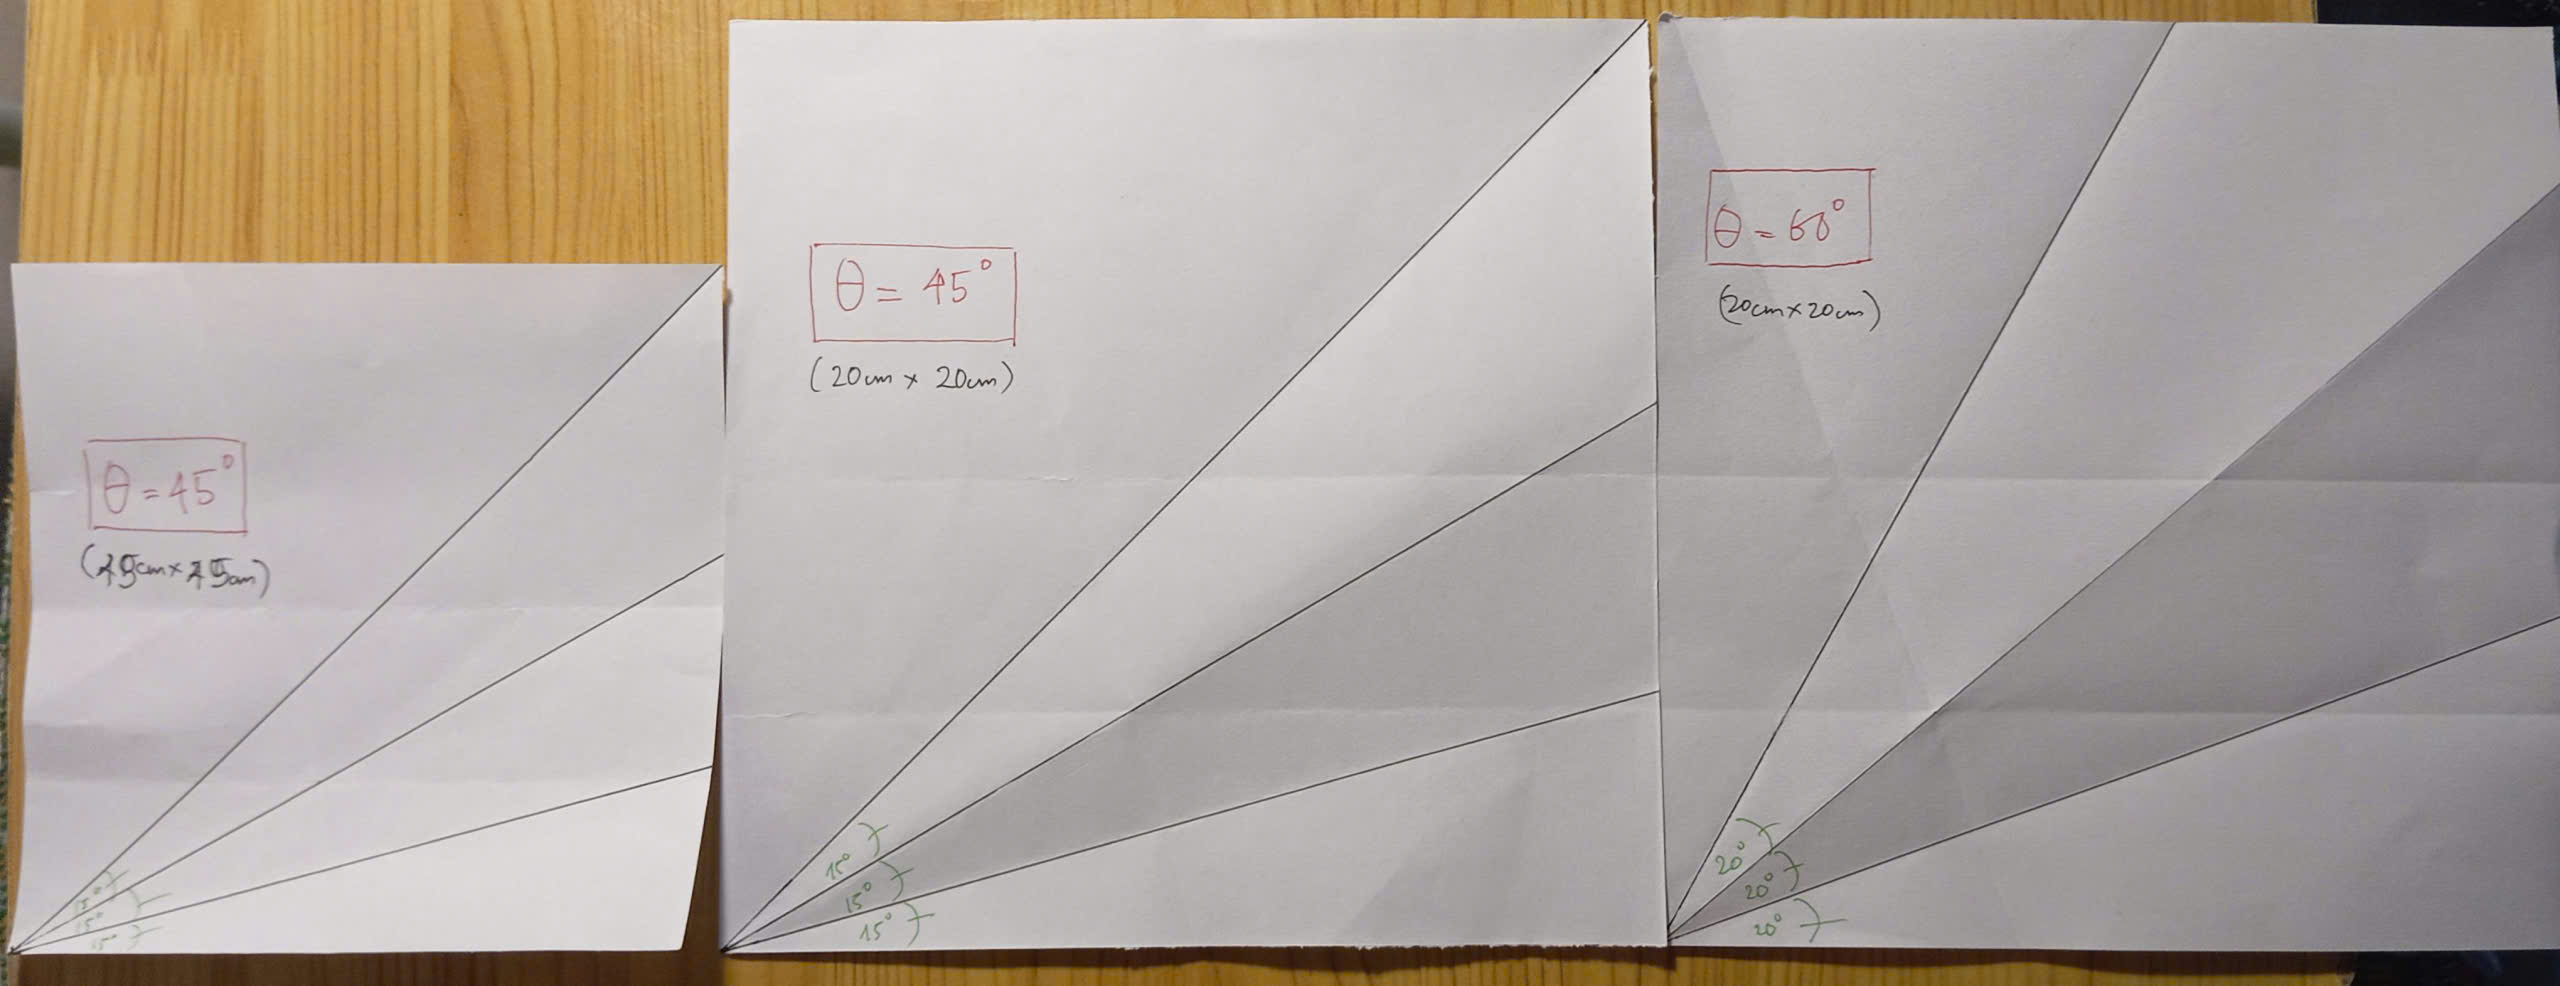
\includegraphics[scale=0.15]{photos/trisectangle.jpg}
\end{center}

\textbf{Nhận xét:} Cách chia này khá chính xác và không thay đổi nếu kích thước khổ giấy 15cmx15cm và 20cmx20cm với góc $\theta=45^\circ$.

\section{Thực nghiệm 2: Dựng tỷ lệ $\sqrt[3]{2}$ (Phương pháp Peter Messer)}

\subsection{Quy trình}
Phương pháp của Peter Messer (1986) cho phép nhân đôi khối lập phương bằng cách xác định tỷ lệ $\sqrt[3]{2}$ trực tiếp trên mép cạnh của tờ giấy hình vuông thông qua Tiên đề 6.

\textbf{Bước 1: Chia tờ giấy thành 3 phần bằng nhau}

Xét tờ giấy hình vuông $ABCD$.
\begin{enumerate}
    \item Chia tờ giấy theo phương ngang thành 3 dải bằng nhau bằng cách ước lượng cuộn mép (hoặc dùng định lý Haga để lấy chính xác tuyệt đối).
    \item Miết tạo hai đường nếp gấp ngang song song: đường nếp dưới $L_1$ và đường nếp trên $L_2$.
\end{enumerate}

\begin{figure}[H]
    \centering
    \begin{tikzpicture}[scale=1.0, >=stealth]
        % Tờ giấy vuông ABCD
        \draw[thick, fill=gray!4] (0,0) rectangle (5.5,5.5);
        \node[below left] at (0,0) {$A$};
        \node[below right] at (5.5,0) {$B$};
        \node[above right] at (5.5,5.5) {$C$};
        \node[above left] at (0,5.5) {$D$};

        % Hai nếp gấp chia 3 phần
        \draw[thick, blue!70, dashed] (0, 1.83) -- (5.5, 1.83);
        \node[font=\footnotesize\bfseries, blue!80!black, fill=white, inner sep=1.5pt] at (5.0, 1.83) {$L_1$};

        \draw[thick, blue!70, dashed] (0, 3.67) -- (5.5, 3.67);
        \node[font=\footnotesize\bfseries, blue!80!black, fill=white, inner sep=1.5pt] at (5.0, 3.67) {$L_2$};

        % Đo kích thước 3 phần bằng nhau
        \draw[<->, gray!80] (-0.3, 0) -- (-0.3, 1.83) node[midway, left, font=\footnotesize] {$\frac{1}{3}$};
        \draw[<->, gray!80] (-0.3, 1.83) -- (-0.3, 3.67) node[midway, left, font=\footnotesize] {$\frac{1}{3}$};
        \draw[<->, gray!80] (-0.3, 3.67) -- (-0.3, 5.5) node[midway, left, font=\footnotesize] {$\frac{1}{3}$};
    \end{tikzpicture}
    \caption{Bước 1: Chia tờ giấy thành 3 dải bằng nhau bằng hai nếp gấp ngang $L_1$ (nếp dưới) và $L_2$ (nếp trên).}
    \label{fig:messer_step1}
\end{figure}

\textbf{Bước 2: Nếp gấp Tiên đề 6}

Cầm đỉnh góc dưới bên trái $A$ và thực hiện gập theo Tiên đề 6:
\begin{itemize}
    \item Đưa đỉnh $A$ sang chạm vào mép đứng bên phải $BC$ tại điểm $A'$.
    \item $L_1$ cắt $AD$ tại E. Đưa E chạm vào $L2$ tại $E'$.
    \item Miết cố định nếp gấp chéo $T$ đi qua $E'A'$
\end{itemize}

\begin{figure}[H]
    \centering
    \begin{tikzpicture}[scale=1.05, >=stealth]
        % --- Khung tờ giấy vuông ABCD ---
        \draw[thick, fill=gray!4] (0,0) rectangle (5.5,5.5);
        \coordinate (A) at (0,0);
        \coordinate (B) at (5.5,0);
        \coordinate (C) at (5.5,5.5);
        \coordinate (D) at (0,5.5);
        
        \node[below left] at (A) {$A$};
        \node[below right] at (B) {$B$};
        \node[above right] at (C) {$C$};
        \node[above left] at (D) {$D$};

        % --- Hai nếp gấp ngang song song L1 và L2 ---
        \draw[thick, blue!50, dashed] (0, 1.83) -- (5.5, 1.83) 
            node[pos=0.92, above, font=\footnotesize, blue!80!black] {$L_1$};
        \draw[thick, blue!50, dashed] (0, 3.67) -- (5.5, 3.67) 
            node[pos=0.92, above, font=\footnotesize, blue!80!black] {$L_2$};

        % --- Điểm ban đầu E = L1 \cap AD và đỉnh A ---
        \coordinate (E) at (0, 1.83);
        \fill[blue!90!black] (E) circle (2.2pt);
        \node[blue!90!black, font=\footnotesize\bfseries, left] at (E) {$E$};
        \fill[black] (A) circle (2.2pt);

        % --- Điểm chạm sau khi gập: E' \in L2 và A' \in BC ---
        % E' nằm trên L2 (y = 3.67)
        \coordinate (E_prime) at (3.5, 3.67);
        % A' nằm trên mép đứng BC (x = 5.5, y chia theo tỷ lệ \sqrt[3]{2}: 5.5 / (1 + 1.2599) \approx 2.43)
        \coordinate (A_prime) at (5.5, 2.43);

        % --- Nếp gấp chéo T đi qua E' và A' ---
        % Đường thẳng nối E'(3.5, 3.67) và A'(5.5, 2.43): y - 2.43 = -0.62 (x - 5.5)
        % Cắt mép trên y = 5.5 tại x \approx 0.55; cắt mép đáy y = 0 tại x \approx 9.4 (vẽ kéo dài trong khung giấy)
        \coordinate (FoldTop) at (0.55, 5.5);
        \coordinate (FoldRight) at (5.5, 2.43);
        \draw[very thick, teal, dashdotted] (FoldTop) -- (FoldRight);
        
        \node[teal!90!black, font=\footnotesize\bfseries, fill=white, inner sep=1.5pt, rounded corners=1pt, rotate=-32] 
            at (2.0, 4.8) {Nếp gấp $T$};

        % Đánh dấu các điểm chạm E' và A'
        \fill[purple!90!black] (E_prime) circle (2.2pt);
        \node[purple!90!black, font=\footnotesize\bfseries, above, fill=white, inner sep=1.5pt, rounded corners=1pt] 
            at (3.5, 3.85) {$E' \in L_2$};

        \fill[red!90!black] (A_prime) circle (2.2pt);
        \node[red!80!black, font=\footnotesize\bfseries, right, fill=white, inner sep=1.5pt, rounded corners=1pt] 
            at (A_prime) {$A' \in BC$};

        % --- Mũi tên uốn cong mô phỏng chuyển động gập ---
        % Gập đỉnh A -> A' \in BC
        \draw[->, thick, red!80!black, bend right=20] 
            (0.15, 0.1) to node[midway, below right, font=\footnotesize] {gập $A \to BC$} (5.35, 2.3);

        % Gập điểm E -> E' \in L2
        \draw[->, thick, blue!80!black, bend left=25] 
            (0.15, 1.95) to node[midway, above left, font=\footnotesize] {gập $E \to L_2$} (3.35, 3.65);
    \end{tikzpicture}
    \caption{Bước 2: Gập đỉnh $A$ sang mép $BC$ tại $A'$, đồng thời đưa điểm $E = L_1 \cap AD$ chạm vào $L_2$ tại $E'$. Nếp gấp $T$ đi qua hai điểm $E'$ và $A'$.}
    \label{fig:messer_step2}
\end{figure}

\textbf{Bước 3: Thu nhận tỷ lệ $\sqrt[3]{2}$ trên mép phải}

Nếu quy ước độ dài đoạn phía dưới $BA'$ làm đơn vị ($1$), thì độ dài đoạn phía trên $A'C$ chính xác bằng căn bậc ba của 2:
\begin{equation}
    \frac{A'C}{BA'} = \sqrt[3]{2} \approx 1{,}25992.
\end{equation}

\begin{figure}[H]
    \centering
    \begin{tikzpicture}[scale=1.0, >=stealth]
        % Tờ giấy vuông ABCD
        \draw[thick, fill=gray!4] (0,0) rectangle (5.5,5.5);
        \node[below left] at (0,0) {$A$};
        \node[below right] at (5.5,0) {$B$};
        \node[above right] at (5.5,5.5) {$C$};
        \node[above left] at (0,5.5) {$D$};

        % Điểm A' trên mép phải
        \coordinate (A_prime) at (5.5, 2.43);
        \fill[red!80!black] (A_prime) circle (2.2pt);
        \node[red!80!black, font=\footnotesize\bfseries, left] at (A_prime) {$A'$};

        % Làm nổi bật 2 đoạn thẳng trên mép phải BC
        % Đoạn dưới: BA' (độ dài 1)
        \draw[line width=2.5pt, blue!80!black] (5.5, 0) -- (A_prime);
        \draw[<->, thick, blue!80!black] (6.0, 0) -- (6.0, 2.43) 
            node[midway, right, font=\small\bfseries] {Đoạn dưới $= 1$};

        % Đoạn trên: A'C (độ dài \sqrt[3]{2})
        \draw[line width=2.5pt, red!80!black] (A_prime) -- (5.5, 5.5);
        \draw[<->, thick, red!80!black] (6.0, 2.43) -- (6.0, 5.5) 
            node[midway, right, font=\small\bfseries] {Đoạn trên $= \sqrt[3]{2} \approx 1{,}2599$};

        % Đường nếp gấp mở mờ để tham chiếu
        \draw[dashed, gray!40] (1.2, 0) -- (5.5, 4.4);
    \end{tikzpicture}
    \caption{Bước 3: Điểm $A'$ chia mép phải của tờ giấy theo đúng tỷ lệ nhân đôi khối lập phương: $\frac{A'C}{BA'} = \sqrt[3]{2}$.}
    \label{fig:messer_step3}
\end{figure}

\subsection{Thực nghiệm}

Thực nghiệm với các khổ giấy 9cmx9cm, 15cmx15cm và 20cmx20cm.
\begin{center}
\includegraphics[scale=0.15]{photos/doublecube.jpg}
\end{center}
\begin{table}[H]
    \centering
    \caption{đo đạc tỉ lệ $A'C / BA'$ theo kích thước giấy}
    \label{tab:paper_size_ratio}
    \small
    \setlength{\tabcolsep}{6pt}
    \renewcommand{\arraystretch}{1.25}
    \begin{tabularx}{\textwidth}{|>{\centering\arraybackslash}m{3.2cm}|>{\centering\arraybackslash}X|>{\centering\arraybackslash}X|>{\centering\arraybackslash}m{2.5cm}|}
        \hline
        \multirow{2}{=}{\centering\textbf{Kích thước giấy}} & \multicolumn{2}{c|}{\textbf{Tỉ lệ $A'C/BA'$ (Phần trên/Phần dưới)}} & \multirow{2}{=}{\centering\textbf{Sai số}} \\
        \cline{2-3}
        & \textbf{Lý thuyết} & \textbf{Thực tế} & \\
        \hline
        $9 \times 9$ & $1.26$ & $1.143$ & $0.117$ \\
        \hline
        $15 \times 15$ & $1.26$ & $1.239$ & $0.021$ \\
        \hline
        $20 \times 20$ & $1.26$ & $1.247$ & $0.013$ \\
        \hline
    \end{tabularx}
\end{table}

\textbf{Nhận xét:} 
\begin{itemize}
  \item Kết quả tương đối chính xác.
  \item Kết quả của khổ 20cmx20cm chính xác hơn khổ 15cmx15cm. Kết quả của khổ 15cmx15cm tốt hơn 9cmx9cm.
\end{itemize}
\begin{center}
{{\bf\fontsize{14pt}{14.5pt}\selectfont 
KẾT LUẬN}}
\end{center}
\addcontentsline{toc}{chapter}{KẾT LUẬN}

Tiểu luận đã làm rõ ranh giới toán học giữa hình học Euclid cổ điển và hình học Origami thông qua hệ thống 7 tiên đề Huzita--Hatori, với các kết quả trọng tâm:

\begin{itemize}
    \item \textbf{Giải mã giới hạn Euclid:} Thước kẻ và compa chỉ giải quyết được các phương trình có bậc mở rộng trường số dạng $2^k$, dẫn đến sự bất khả thi đối với bài toán chia ba góc và nhân đôi khối lập phương (vốn đòi hỏi giải phương trình bậc ba tối tiểu).
    \item \textbf{Bản chất toán học của Tiên đề 6:} Thao tác đưa đồng thời hai điểm chạm vào hai đường thẳng tương đương với việc dựng tiếp tuyến chung của hai đường parabol. Cơ chế này mở rộng bậc trường số lên dạng $2^a \cdot 3^b$, cho phép tìm nghiệm thực của phương trình bậc ba trực tiếp qua tương tác vật lý mà không cần công thức đại số phức tạp.
    \item \textbf{Giá trị thực nghiệm:} Quy trình gập của Abe Hisashi và Peter Messer đã chứng minh tính khả thi tuyệt đối trên giấy thực tế. Bảng số liệu đo đạc cho thấy sai số thực nghiệm hoàn toàn nằm trong ngưỡng cho phép ($\approx \SI{0.39}{\percent} - \SI{1.33}{\percent}$), xuất phát chủ yếu từ độ co giãn và độ dày của vật liệu giấy.
\end{itemize}

Vượt ra ngoài một nghệ thuật tạo hình dân gian, Origami chính là một hệ tiên đề toán học chặt chẽ. Sự giao thoa giữa những nếp gấp mộc mạc và cấu trúc đại số trừu tượng đã minh chứng rằng: giới hạn của một bài toán đôi khi không nằm ở bản chất hình học, mà chỉ nằm ở công cụ ta lựa chọn để tiếp cận nó.
\addcontentsline{toc}{chapter}{Tài liệu tham khảo}

\begin{thebibliography}{99}
\bibitem{Lang}
Robert J. Lang, Origami Design Secrets: Mathematical Methods for an Ancient Art, CRC Press.
\bibitem{Hull}
Thomas Hull, Project Origami: Activities for Exploring Mathematics, CRC Press.
\bibitem{Abe}
Hisashi Abe, Abe's Theorem: Trisection of an Angle by Origami, 1980.
\bibitem{Messer}
Peter Messer, Cube Doubling by Origami, British Origami, 1986.

\end{thebibliography}




\end{document}

\end{document}

